\documentclass[a4paper, twoside]{article}
\usepackage{geometry} \geometry{top=30mm, bottom=25mm, inner=20mm, outer=20mm}
\usepackage[linktoc=all]{hyperref}
\hypersetup{
	bookmarksopen=true,
	bookmarksdepth=3,
	colorlinks=true,
	citecolor=blue,
	linkcolor=[rgb]{0.6,0,0}}
\usepackage{graphicx}
\setlength{\abovecaptionskip}{0pt}
\usepackage{amssymb,amsmath,physics}
\begin{document}

\title{Versuchsdurchführung zu Dopplerfreie Sättigungsspektroskopie von Rubidium}
\author{Anna-Maria Pleyer}
\date{\today}
\maketitle
\section{Versuchsaufbau realisieren}
\subsection{Bereits aufgebaut} 
$\Rightarrow$ keine Veränderung notwendig
\begin{itemize}
    \item Laser
    \item lineare Polarisator
    \item Spiegel S1 und S2 
    \item $\frac{\lambda}{2}$ Plättchen
\end{itemize}
\subsection{Justage}
Nach Abbildung:
\begin{figure}[h]
    \centering
    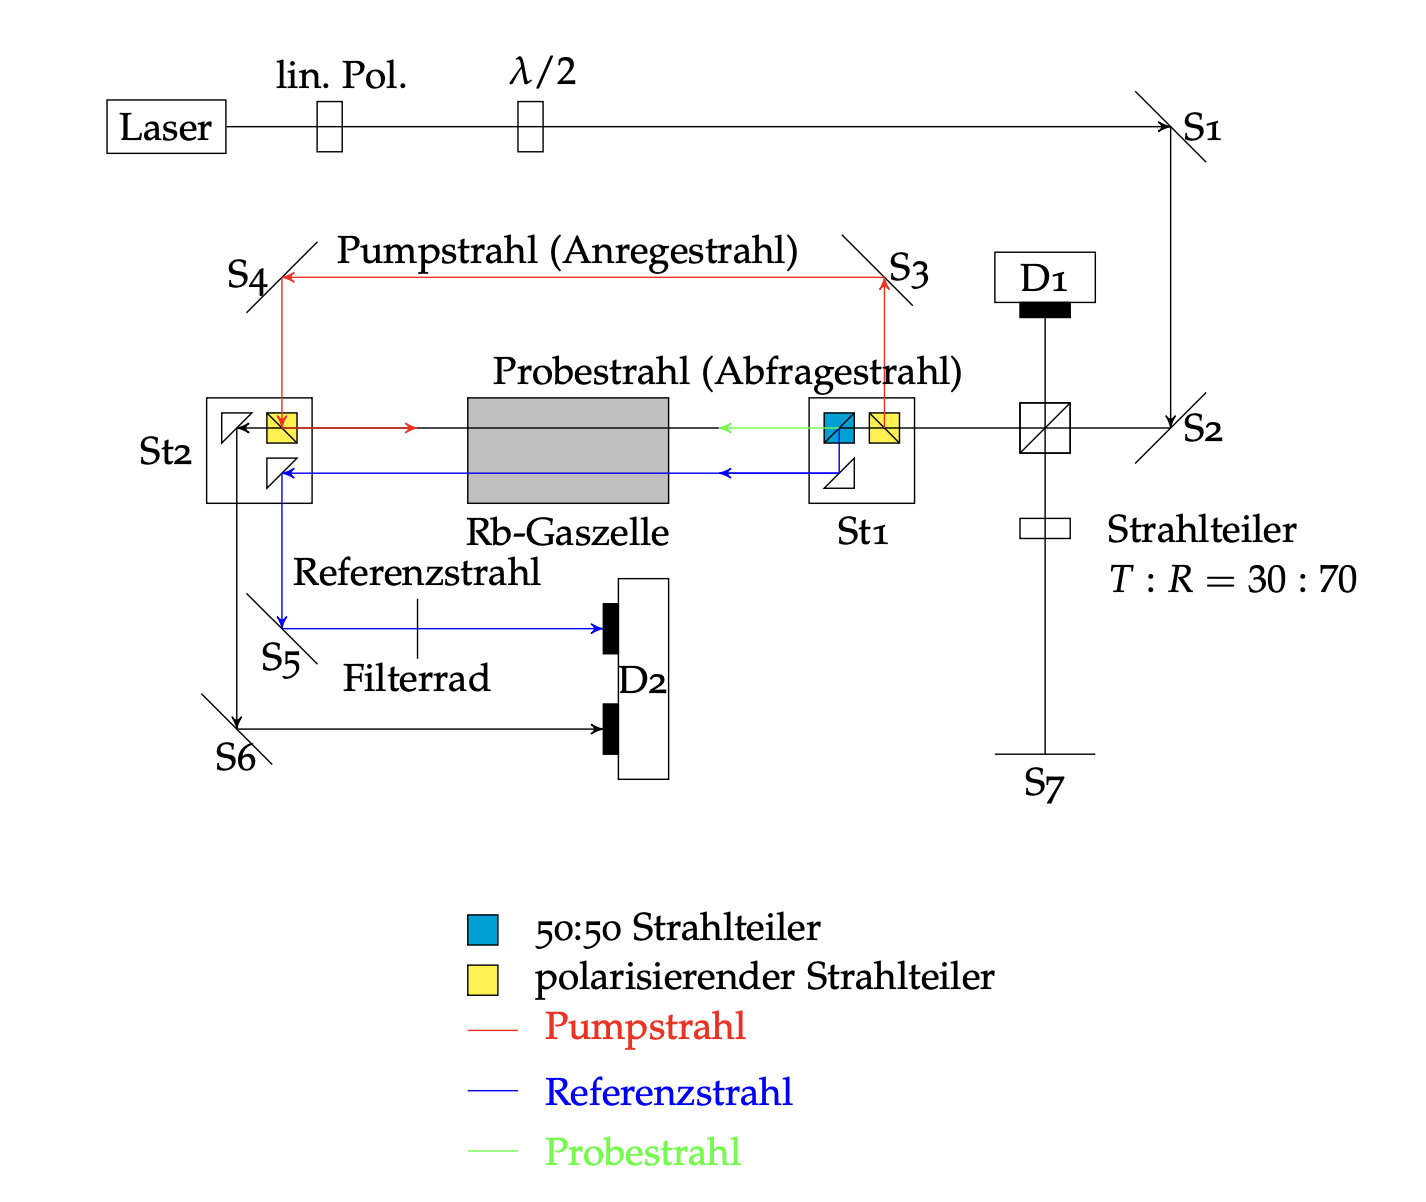
\includegraphics[scale=0.5]{Bilder/Abbildung3.png}
    \caption{Versuchsaufbau}
   \end{figure}
\newpage
\begin{itemize}
    \item[a)] S3 und S4 justieren
    \begin{itemize}
        \item Höhe: 12\,cm
        \item auf Lochreihe stellen
        \item ca. 45° zum einfallenden Strahl
        \item siehe Abbildung 2
    \end{itemize} 
    \begin{figure}[h]
        \centering
        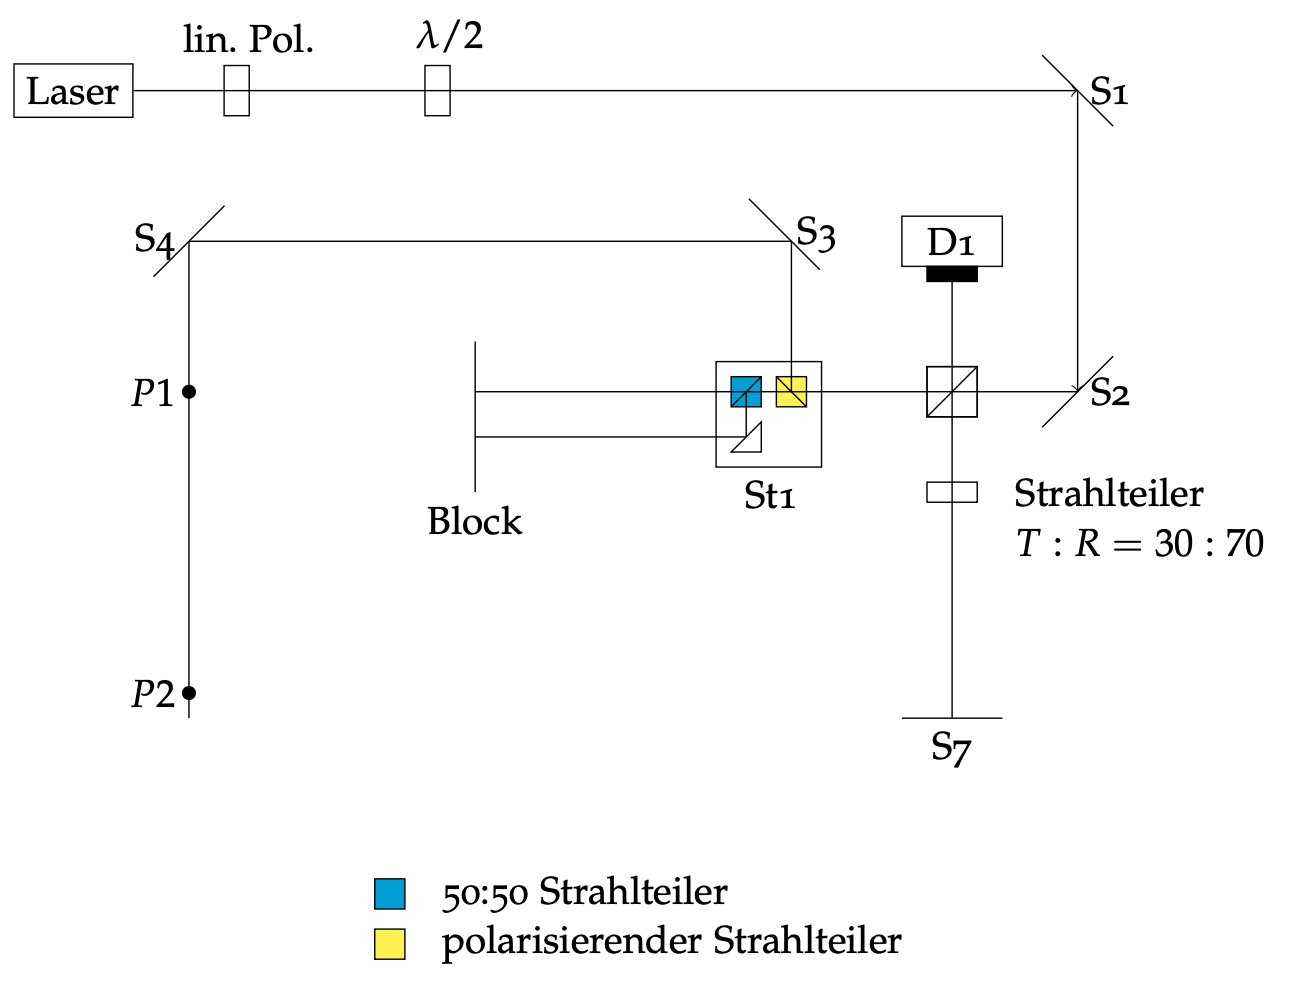
\includegraphics[scale=0.4]{Bilder/Abbildung4.png}
        \caption{Justierung von S3 und S4}
       \end{figure}
    \item[b)] Strahl mit Justierspitze ausrichten
    \begin{itemize}
        \item Auswahl von zwei Positionen auf Lochreihe
        \item P1: Stelle wo zweiter Strahlenteile St2 stehen soll
        \item P2: so weit wie möglich entfernt
    \end{itemize} 
    \item[c)] Justage von S3 auf P1 und S4 auf P2 abwechselnd \\
    $\Rightarrow$ Justierspitze muss genau gestroffen werden
    \item[d)] Falls schwacher Laser: Intensität mithilfe des $\frac{\lambda}{2}$ Plättchen erhöhen 
    \item[e)] Strahlenteiler St2 einbauen
    \begin{itemize}
        \item nach Abbildung 1 einbauen
        \item optische Elemente müssen vom Strahl mittig getroffen werden 
        \item Strahlenteiler justieren $\Rightarrow$ Strahlenteiler soll nicht verkippen
        \begin{itemize}
            \item Pumpstrahl blocken
            \item Pumpstrahl per Rückflexion auf S4 justieren
        \end{itemize}
    \end{itemize}
  \item[f)] Pump- und Probestrahl überlagern
  \begin{itemize}
      \item zwei Irisblenden[I1 und I2] (Höhe Mittelpunkt 12\,cm) zwischen St1 und St2 einbauen
      \item S3 auf I1 justieren 
      \item S4 auf I2
      \item Vergleiche Abbildung 3
  \end{itemize} 
  \begin{figure}[h]
    \centering
    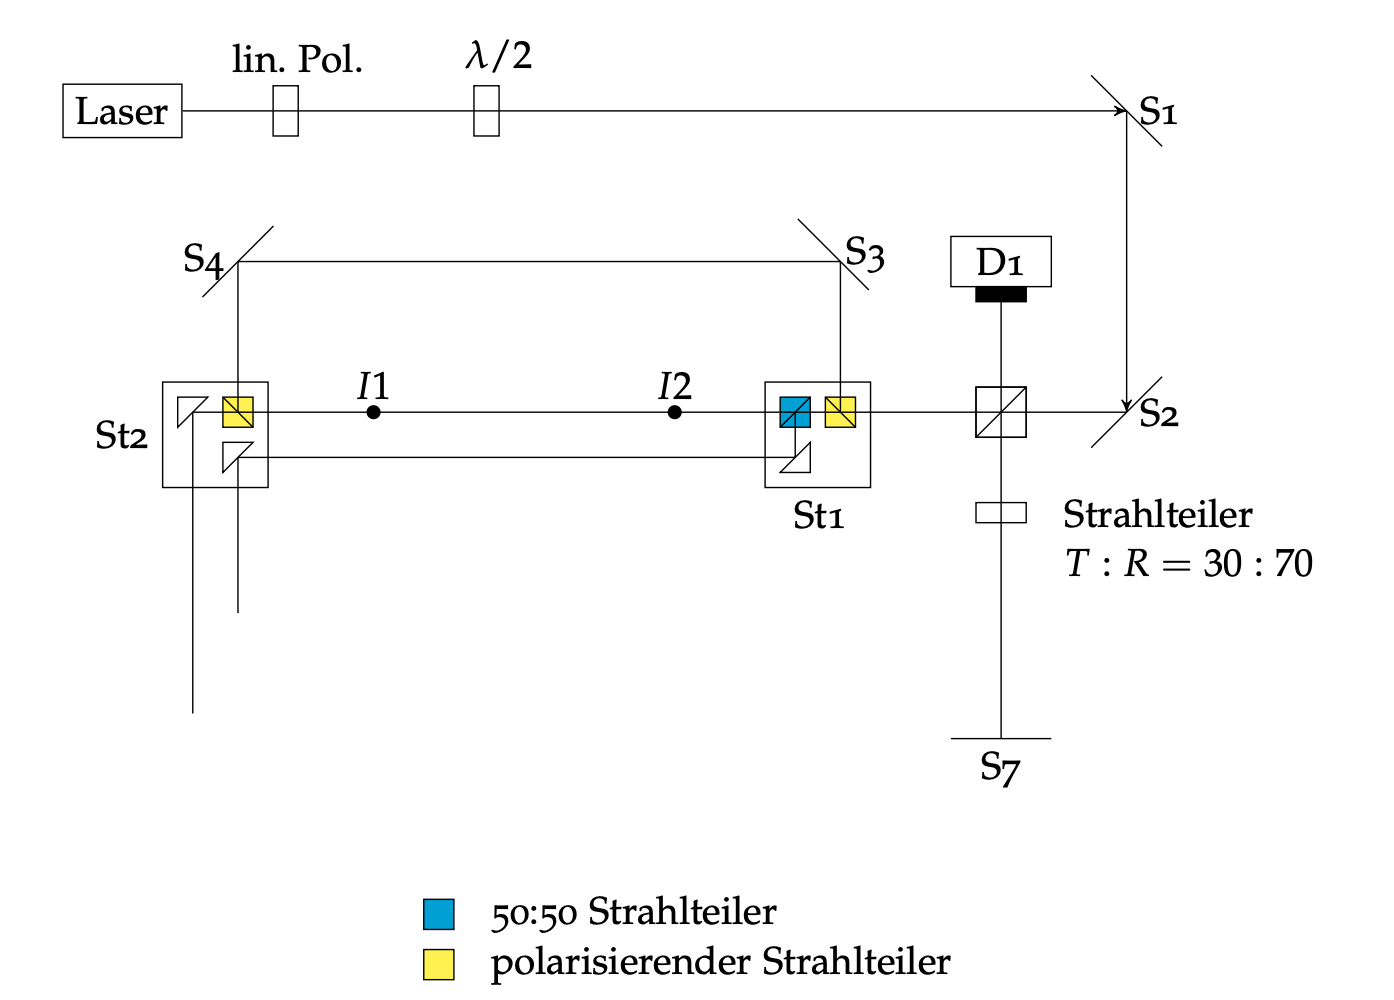
\includegraphics[scale=0.4]{Bilder/Abbildung5.png}
    \caption{Überlagerung von Pump- und Probestrahl}
   \end{figure}
   \newpage
  \item[g)] S5, S6 und Detektor D2 wie in Abbildung 1 aufbauen\\
  $\Rightarrow$ Strahlen müssen Detektor mittig treffen
  \item[h)] Gaszelle einsetzen
  $\Rightarrow$  beide Strahlen zwischen St1 und St2 müssen gerade und parallel durch Gaszelle verlaufen
\end{itemize}
\subsection{Hinweis zur Justage}
Laserstrahl läuft über einen Spiegel hinaus:
\begin{itemize}
    \item  Spiegel wshl. zu weit neben der gewünschten Lochreihe
    \item Spiegeloberfläche (und nicht Halterung) müssen auf der richtigen Lochreihe stehen
    \item  Spiegeloberfläche in 45° zum einfallenden Strahl 
    \item Spiegel soltte mit Laserstrahl mittig getroffen werden
\end{itemize}
\section{Abstimmung der Strahlintensitäten}
\begin{itemize}
    \item mithilfe des $\frac{\lambda}{2}$ Plättchen und Filterrad
    \item Intensität Referenzstrahl = Intensität des parallelen Probestrahl (ohne Pumpstrahl)
    \item Pumpstrahl stärker als Probestrahl 100:1
    \item Intensitäten mit Messprogram ablesebar
    \item Veränderung der Intensitäten mithilfe des Filterrades
\end{itemize}

\section{Überprüfung der Detektoren und Gaszelle}
\begin{itemize}
    \item Gaszelle muss am Heizer (richtig) angeschlossen sein
    \item Detektor mit Strom versorgen
    \item Detektor an aio-ai4 des NI-USB 6002 AD-Interface anschließen
\end{itemize}
\section{Messprogramm}
\begin{itemize}
    \item Zeeman-op
    \item Funktioniert nur wenn ... eingeschaltet:
    \begin{itemize}
        \item Laser
        \item Heizelement der Gaszelle\\ 
        $\Rightarrow$ Temperature Controller
        \item programmable DC power Supply
        \item Function Arbitrary Waveform Generator
    \end{itemize}
\end{itemize}
\subsection{Hinweise zum Messprogramm}
\begin{itemize}
    \item Linke Seite: Auswahl der Kanäle
    \item Registerkarten
    \begin{itemize}
        \item Laserpower
        \begin{itemize}
            \item rechtes Feld: Speicherung der Messung
            \item Einstellung der \textit{Scan-range} \\
                $\Rightarrow$ Bereich welchen der Laserstrahl durchlaufen soll
            \item Einstellung der \textit{Scan-steps} \\
                $\Rightarrow$ Wie viele Punkte sollen in dem Bereich aufgenommen werden?\\
                $\Rightarrow$ Maximum 2000 bei einer Messreihe
            \item Einstellung der \textit{dt/pixel}\\
            $\Rightarrow$ Zeit pro Messpunkt während der Messung \\
            $\Rightarrow$ Wert zwichen 100 und 200 bei einer Aufnahme einer Messreihe 
        \end{itemize}
        \item Adjust\\
        $\Rightarrow$ Eingangsignal in Echtzeit\\
        $\Rightarrow$ wichtig für Intensitätsanpassung
    \end{itemize}
\end{itemize}
\subsection{Hinweise zur Signalverbesserung}
\begin{itemize}
    \item Modensprung = Schlagartiger Sprung der Wellenlänge
    \item Aufnahme des doppelverbreiterten Spektrum innerhalb von 2 Modensprüngen\\
    $\Rightarrow$ 4 Linien innerhalb 2 Modensprünge müssen klar voneinander unterscheidbar sein\\
    $\Rightarrow$ Verschiebung der Modensprünge: Lasertemperatur [Veränderung zwischen 21° und 23° in 0,2° Schritten]
    \item EXAKTE Überlagerung von Pump- und Probestrahl
    \item Sättigung des Detektors: \\
    $\Rightarrow$ Verringerung der Intensität (vor dem Detektor abschwächen, damit keine Veränderung im Versuchsaufbau)
    \item Falls keine Hyperfeindips: Anpassung der Intensitäten 
\end{itemize}
\newpage
\section{Aufgaben}
\textbf{Allgemein}
\begin{itemize}
    \item FPI Signal BEI JEDER MESSUNG mitaufnehemen
    \item Kanäle notieren
    \item Jeweils für Gaszellentemperatur von 23° bis 60° messen
\end{itemize}
\textbf{Messungen}
\begin{itemize}
    \item[1.] Ausschnitt zwischen 2 Modensprüngen (alle 4 Linien müssen erkennbar sein)
    \item[2.] Die einzelnen Linien messen (Linien BENENNEN)
    \item[3.] Ausschnitt zwichen zwei Modensprüngen bei Lasertemperatur 40° 
\end{itemize}
\end{document}